\documentclass[../main.tex]{subfiles}
% b = k × λ ÷ sin(α)
%   α = 30°; λ = 530nm
%   -> b = 1500nm

\subsection{Versuchsaufbau}

% 4.1.1 Figuren
\begin{figure}[ht]
    \begin{subfigure}[b]{0.5\textwidth}
        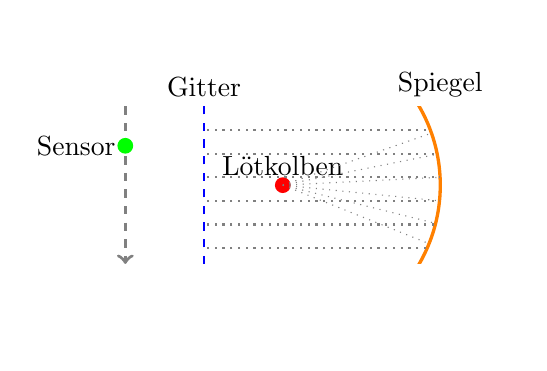
\begin{tikzpicture}
            %\draw[step=1] (-3,-2) grid (4,2);

            % Spiegel
            \begin{scope}
                \clip (2,1) rectangle (4,-1);
                \draw (1,0)[orange,very thick] circle (2);
            \end{scope}
            \draw (3,1) node[black,anchor=south] {Spiegel};
            
            \fill[red] (1,0) circle (0.1) node[black,anchor=south] {Lötkolben};
            
            % EM-Strahlungen
            \begin{scope}
                \clip (1,0) circle (2);
                \clip (0,-1) rectangle (3,1);
                \foreach \i in {0.3,0.6,...,2} {
                    \draw[gray,dotted] (1,0) -- (3,{\i-1.1}); % Abgegeben
                    \draw[gray,dotted,thick] (4,{\i-1.1}) -- (0,{\i-1.1}); % Reflektiert
                }
            \end{scope}
            
            \draw[blue,thick,dashed] (0,-1) -- (0,1) node[black,anchor=south] {Gitter};
            
            \draw[very thick,gray,dashed,->] (-1,1) -- (-1,-1);
            \fill[green] (-1,0.5) circle (0.1cm) node[black,anchor=east] {Sensor};
        \end{tikzpicture}
        \caption{Schematischer Versuchsaufbau}
        \label{fig:versuchsaufbau-schematisch}
    \end{subfigure}
    \begin{subfigure}[b]{0.5\textwidth}
        \includegraphics[width=\textwidth]{23c-spektrometer-600-pro-mm.png}
        \caption{Experiment}
        \label{fig:versuchsaufbau-foto}
    \end{subfigure}
    \caption{Aufbau}
    \label{fig:experiment_aufbau}
\end{figure}

% Bilder:
%   - loetkolben
%   - hg-lampe
%   - spiegel
%   - sensor
%   - gitter

% 4.1.2 Erklärung schematisch
Der Aufbau ist wie folgt (Abb. \ref{fig:versuchsaufbau-schematisch}): Ein lötkolben gibt eine punktförmige Infrarotstrahlung ab, welcher vom Spiegel als Parallelstrahl zum Gitter reflektiert wird. Die gebeugten Wellen werden vom Sensor dedektiert.

\subsection{Ergebnisse}

\begin{figure}[ht]
    \centering
    \begin{subfigure}[b]{0.3\textwidth}
        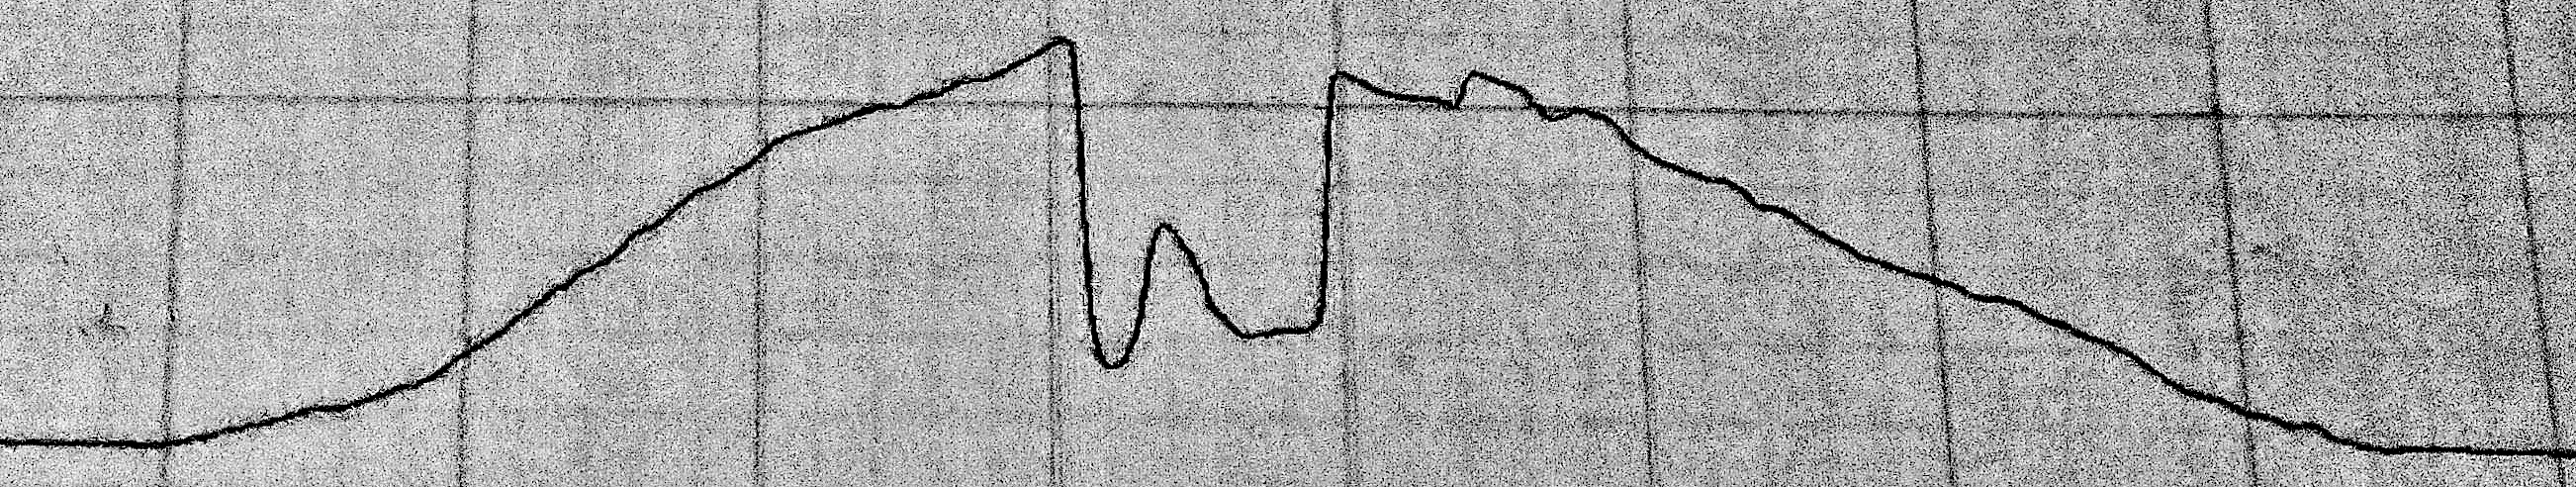
\includegraphics[width=\textwidth]{experiment/spectra/21c-diagramm-600-pro-mm.png}
        \caption{600 Linien / mm}
    \end{subfigure}
    \begin{subfigure}[b]{0.3\textwidth}
        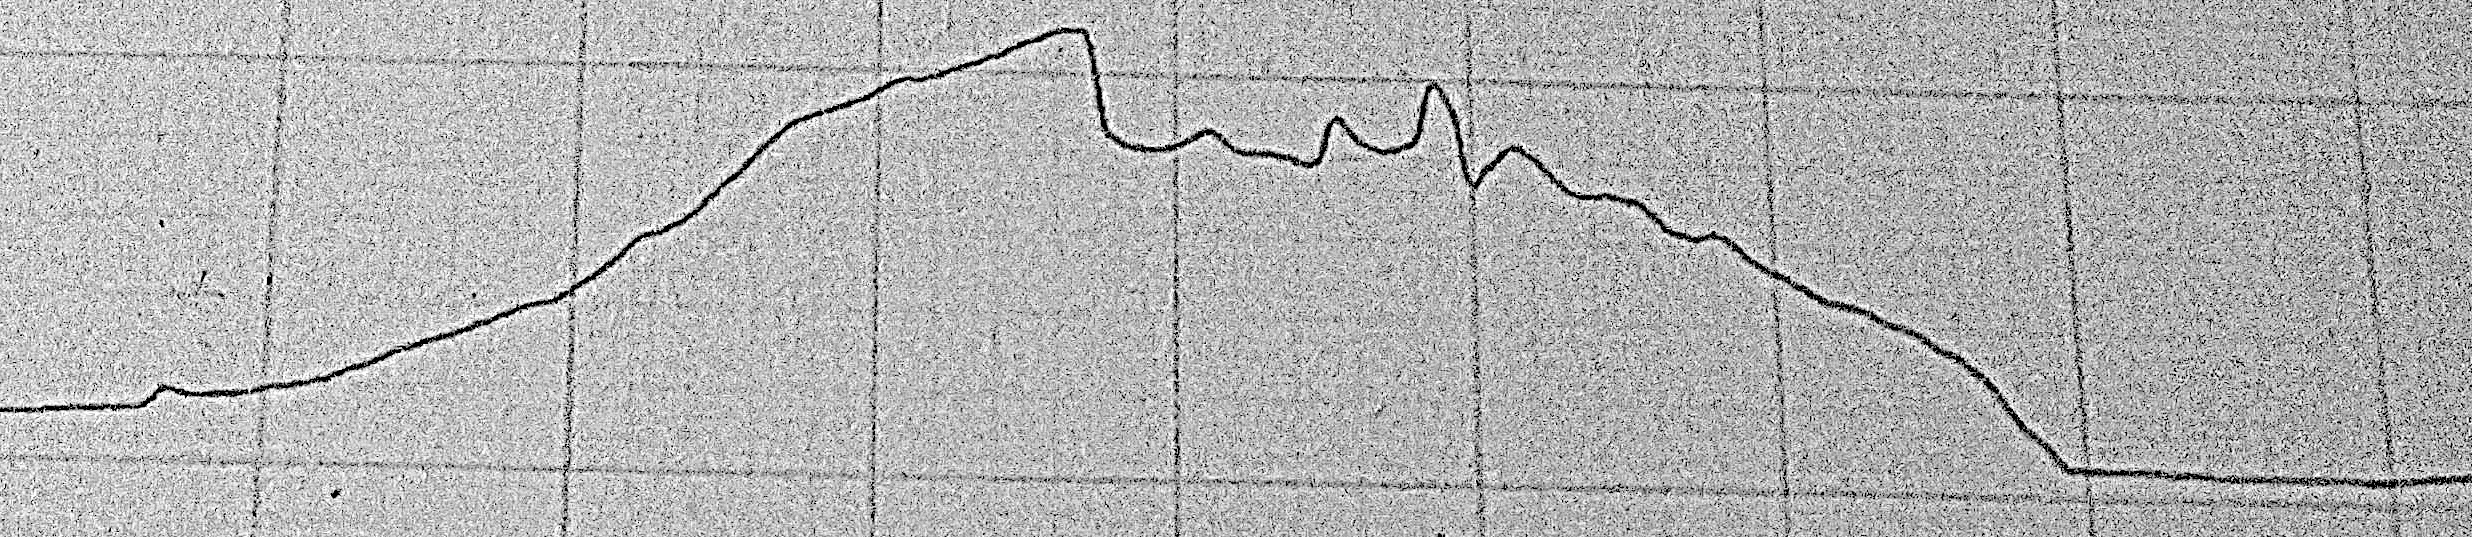
\includegraphics[width=\textwidth]{experiment/spectra/27c-diagramm-leypold.png}
        \caption{Leybold}
    \end{subfigure}
    \begin{subfigure}[b]{0.3\textwidth}
        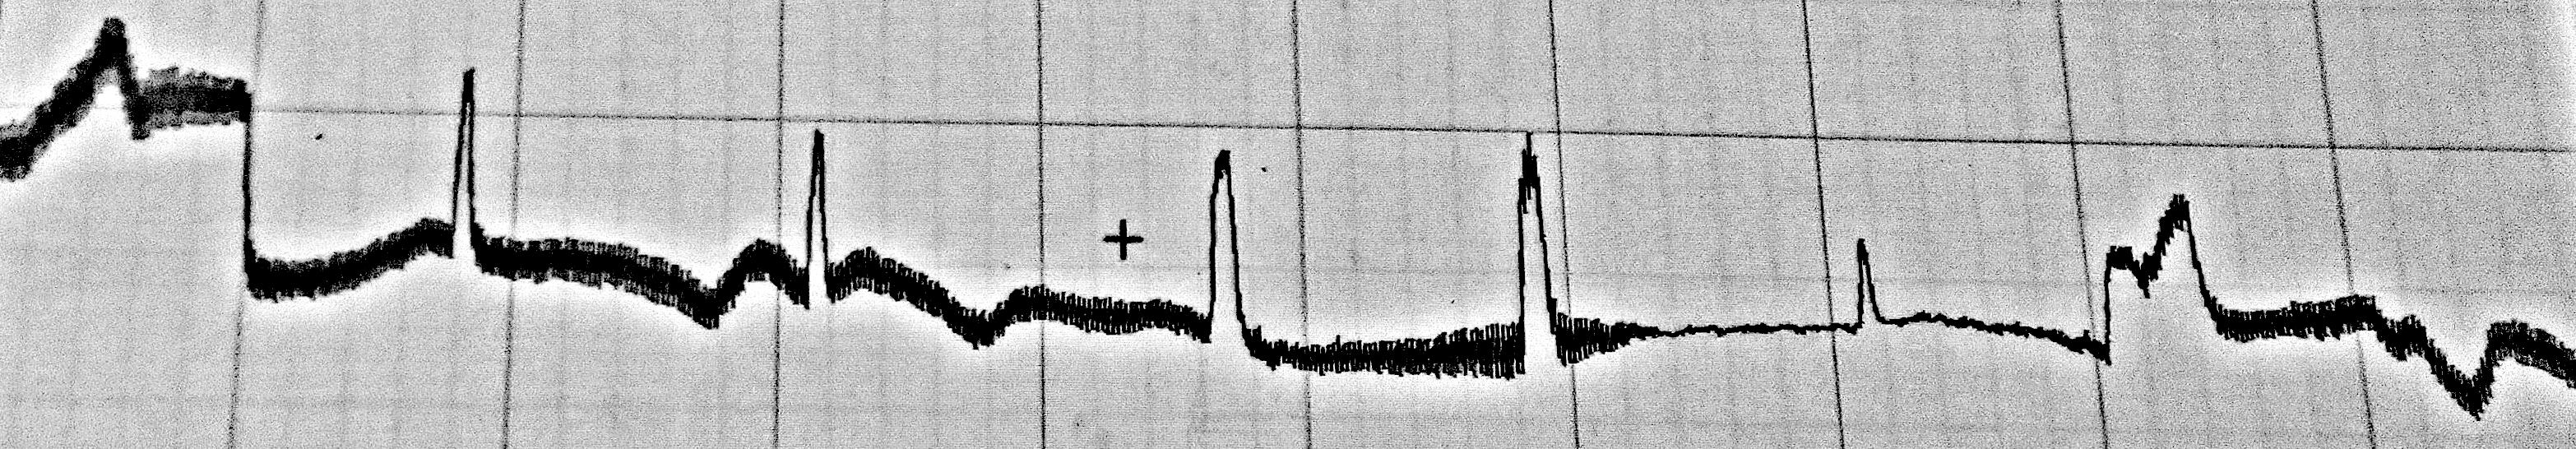
\includegraphics[width=\textwidth]{experiment/spectra/30c-diagramm-reflexionsgitter.png}
        \caption{Reflexionsgitter}
    \end{subfigure}
    \caption{Spektra verschiedener Gitter}
\end{figure}

% Diagramme
% Fehler
